\documentclass[11pt]{article}
\usepackage[letterpaper,margin=1in]{geometry}
\usepackage{amsmath,amssymb,amsthm}
\usepackage{graphicx}
\usepackage{booktabs}
\usepackage{array}
\usepackage{float}
\usepackage[ruled]{algorithm}
\usepackage[font=small,labelfont=bf]{caption}
\usepackage{xcolor}
\usepackage[colorlinks=true,allcolors=blue]{hyperref}

\graphicspath{{figs/}}

\newcommand{\sigm}{\sigma}
\newcommand{\E}{\mathbb{E}}
\newcommand{\R}{\mathbb{R}}
\newcommand{\cB}{\mathcal{B}}
\newcommand{\cU}{\mathcal{U}}
\newcommand{\cA}{\mathcal{A}}
\newcommand{\cI}{\mathcal{I}}
\newcommand{\cW}{\mathcal{W}}
\newcommand{\cP}{\mathcal{P}}
\newcommand{\cN}{\mathcal{N}}
\newcommand{\nexp}{n_{\mathrm{exp}}}
\newcommand{\Fit}{\mathrm{Fit}}
\newcommand{\Route}{\mathrm{Route}}
\newcommand{\Filter}{\mathrm{Filter}}
\newcommand{\Acquire}{\mathrm{Acquire}}
\DeclareMathOperator*{\argmax}{arg\,max}
\DeclareMathOperator{\argsort}{argsort}

\theoremstyle{plain}
\newtheorem{proposition}{Proposition}
\newtheorem{theorem}{Theorem}
\theoremstyle{definition}
\newtheorem{definition}{Definition}
\newtheorem{problem}{Problem}
\theoremstyle{remark}
\newtheorem{remark}{Remark}

\title{\textbf{Maintaining a Living Benchmark\\
with Item Response Theory}}
\author{}
\date{}

\begin{document}
\maketitle
\vspace{-3.2em}

\begin{abstract}
Benchmarks for modern AI models face two problems. First, they usually score models
by raw accuracy, even though test questions differ greatly in difficulty: a model
that passes hard questions and one that passes easy ones can receive the same score.
Second, a fixed benchmark loses value over time. As models improve, questions that
once separated them become ones every model passes, and the leaderboard flattens.
This paper takes item response theory as the answer to the first problem and
addresses the second. We measure a question's value by how much it tells us about
today's models, and prove a simple law: a question is most useful when its
difficulty matches the average model, and its value then falls off exponentially as
models grow past it, at a rate set by how fast the field improves. Keeping a
benchmark useful is therefore a moving target. We give an algorithm that tracks it.
Like the SAT and GRE, which maintain a library of questions rather than one permanent
test, it keeps a fixed set of anchor questions to measure progress on a stable scale,
re-estimates each question's difficulty from model answers, retires questions that
have become too easy, and adds new hard ones. We prove this algorithm keeps the
benchmark as informative as possible at every point in time, as long as new hard
questions are added at least as fast as the models improve. Synthetic experiments
confirm both the law and the algorithm. Finally, with scores made stable over time,
a simple average win-rate names a clear overall winner.
\end{abstract}

\section{Introduction}

Benchmarks are how the field keeps score. A new model is judged by where it lands
on a leaderboard, and a leaderboard is, at bottom, a test: a fixed set of questions,
a count of how many each model gets right. It is worth asking how the people who
design tests for a living handle the same job. A useful example comes from
standardized tests such as the SAT and GRE. These tests do not score a student by raw
accuracy alone. Two students may both answer 90 of 100
questions correctly, but if one of them answered harder questions, the two should not
receive the same estimate of ability. Item response theory, the framework behind
these tests, estimates ability from both how many questions a student answers
correctly and how hard those questions were. Just as important, the SAT and GRE do
not rely on one permanent set of questions. They maintain a library of questions that
is updated over time, so that the test keeps separating students as the population
changes and scores from different years stay comparable.

Evaluating modern AI models presents an analogous problem, in two parts. The first
is difficulty. A benchmark's questions vary substantially in how hard and how
informative they are, yet the standard leaderboard score averages over them as though
they were equivalent. On a reasoning benchmark, for example, many questions are
answered correctly by every model in the field, and a model does well on them simply
by matching what everyone else already knows; a few require much more, and only
those tell the strong models from the rest. Averaging over both hides the questions
that actually test a model.

The second part is time, and it is the subject of this paper. Benchmarks have short
useful lives. A test that cleanly separated last year's models often fails to
separate this year's. The usual explanation---``the benchmark is saturated''---names
the symptom, not the cause. The cause is that the models keep improving, so questions
that once sat in the middle of the field, where they tell models apart best, end up
below it, where everyone passes and nothing is learned. The ruler did not shrink; the
things it measures outgrew it. This is different from what is usually called drift,
where a deployed model gets worse as the world moves away from its training data.
Here the models get better, and it is the benchmark that loses resolution. We call
this \emph{capability drift} and ask a simple question: how should a benchmark be
maintained so that it keeps ranking a field that is always improving?

We answer it in three steps, using the item-response view throughout: each model has
an ability, each question (an \emph{item}) has a difficulty, and each model--question
pair is recorded as pass or fail. First, we say what a question is worth at a given
time and show how fast that worth decays (\S\,\ref{sec:setup}). Second, we state the
maintenance task as a precise goal: keep the benchmark as informative as possible at
every round (Problems~\ref{prob:one} and~\ref{prob:online}, also in
\S\,\ref{sec:setup}). Third, we give an algorithm and prove it meets that goal under
a clear condition (\S\,\ref{sec:algo}). Synthetic experiments confirm the theory
(\S\,\ref{sec:exp}), and we close by discussing how to name a single winner
(\S\,\ref{sec:disc}). Together these turn a benchmark from a fixed leaderboard into a
living evaluation system, one that stays fair, informative, and comparable over time
as the field advances.

\paragraph{Contributions.} (i) A definition of benchmark value and a decay law: each
question's value is single-peaked in time and decays like $e^{-rt}$, where $r$ is the
rate of progress (\S\,\ref{sec:setup}). (ii) The maintenance task stated as an
optimization problem over time (Problems~\ref{prob:one} and~\ref{prob:online}).
(iii) An algorithm that maintains the benchmark from a single pool of answers, with a
theorem showing it stays near-optimal at all times exactly when new hard questions
arrive as fast as the field improves (\S\,\ref{sec:algo}). (iv) Synthetic experiments
(\S\,\ref{sec:exp}) and a comparison of single-winner rules (\S\,\ref{sec:disc}).

\paragraph{Relation to a companion paper.} A companion paper studies how to read a
model's ability cleanly from many sub-benchmarks at a \emph{single} time. This paper
is its time-varying counterpart, and reuses two of its ideas: linking scores through
shared questions, and estimating question difficulty from answers. The companion
paper removes the effect of \emph{which} questions are asked; this paper removes the
effect of \emph{when} they are asked. The paper is self-contained: all tools we use
are defined below.

\section{Setup and the Maintenance Problem}
\label{sec:setup}

We set up the model (\S\,\ref{sec:model}), describe how the field of models moves over
time (\S\,\ref{sec:field}), define a question's value and prove the decay law
(\S\,\ref{sec:value}), and state the maintenance goal as an optimization problem
(\S\,\ref{sec:problem}).

\subsection{Models, questions, and ability}
\label{sec:model}

There are $M$ models, indexed by $j\in\{1,\dots,M\}$; model $j$ has an ability
$\theta_j\in\R$. Questions (\emph{items}) are drawn from a universe $\cU$;
item $i$ has a difficulty $b_i\in\R$. We use the one-parameter (Rasch) model: model
$j$ answers item $i$ correctly with probability
\begin{equation}
P(U_{ij}=1)=\sigm(\theta_j-b_i),\qquad \sigm(z)=\frac{1}{1+e^{-z}},
\label{eq:rasch}
\end{equation}
so an item is fully described by its difficulty. The information a single item
carries about a model's ability is
\begin{equation}
I_b(\theta)=\sigm(\theta-b)\bigl(1-\sigm(\theta-b)\bigr)\le\tfrac14,
\label{eq:info}
\end{equation}
which is largest when the difficulty matches the ability ($b=\theta$) and falls off
like $e^{-|\theta-b|}$ on either side: a question is most telling for models near its
own level, and nearly useless for models that almost always pass or almost always
fail it. Given a model's answers to items of known difficulty, we estimate its
ability by the standard penalized fit
\begin{equation}
\hat\theta_j=\argmax_{\theta}\sum_i\Bigl[U_{ij}\log\sigm(\theta-b_i)
+(1-U_{ij})\log\bigl(1-\sigm(\theta-b_i)\bigr)\Bigr]-\frac{\theta^2}{2\tau^2},
\label{eq:fit}
\end{equation}
which has a unique solution.

\paragraph{Notation.} $|S|$ is the size of a set $S$, and $S\setminus S'$ is the set
of elements in $S$ but not $S'$. A \emph{bank} $\cB\subset\cU$ is a finite set
of items, which we treat as a set of difficulties. A subscript $t$ marks a round-$t$
quantity, and a hat marks an estimate.

\subsection{The moving field of models}
\label{sec:field}

The new feature of our setting is time. At round $t=0,1,2,\dots$ the field of models
is described by a distribution $\cP_t$ of abilities, with density $\rho_t$, mean
$\mu_t$, and spread $s_t$. We write $\E_t$ for an average over $\cP_t$.
\emph{Capability drift} is the upward motion of this distribution. We take the mean
to rise at a steady rate and the spread to stay fixed,
\begin{equation}
\mu_t=\mu_0+r\,t,\qquad s_t\equiv s,
\label{eq:drift}
\end{equation}
where $r>0$ is the \emph{drift rate}, in ability units per round. (This linear form
is the natural one: capability tends to grow about linearly on the logit ability
scale used here.) The goal each round is to rank the current field from the
estimates $\hat\theta_j$.

\subsection{The value of a question, and how it decays}
\label{sec:value}

A question is useful insofar as it tells apart the models being tested \emph{now}.
The right measure is the information~\eqref{eq:info}, averaged over the current
field.

\begin{definition}[Value]
\label{def:value}
The \emph{value} of item $i$ at round $t$ is its average information about a current
model,
\begin{equation}
v_t(b)=\E_t\bigl[I_b(\theta)\bigr]=\int I_b(\theta)\,\rho_t(\theta)\,d\theta,
\label{eq:value}
\end{equation}
and the value of a bank $\cB$ is the sum $V_t(\cB)=\sum_{i\in\cB}v_t(b_i)$.
\end{definition}

Value is the benchmark's measuring power for the current field. It obeys a simple law.

\begin{proposition}[Decay law]
\label{prop:decay}
Let the field be $\cP_t=\cN(\mu_t,s^2)$. Once the field has risen above a question
($\mu_t-b\gtrsim 2$), its value is approximately
\begin{equation}
v_t(b)\;\approx\;e^{s^2/2}\,e^{-(\mu_t-b)}.
\label{eq:decay}
\end{equation}
With $\mu_t=\mu_0+rt$ this means $v_t(b)\propto e^{-rt}$: the value of a passed
question decays exponentially in time at the drift rate $r$, halving every
$\ln 2/r$ rounds. Before that, the value \emph{rises} as the field approaches the
question, and it peaks exactly when $\mu_t=b$.
\end{proposition}

\begin{proof}
For $\theta-b$ large, $I_b(\theta)\approx e^{-(\theta-b)}$. Averaging over
$\theta\sim\cN(\mu_t,s^2)$ and using $\E[e^{-(\theta-\mu_t)}]=e^{s^2/2}$ gives
$v_t(b)\approx e^{-(\mu_t-b)}e^{s^2/2}$. This needs the field to sit above the
question, so the approximation describes the decay, not the rise. That $v_t(b)$ peaks
at $\mu_t=b$ follows because, as a function of $\mu_t$, its derivative changes sign
there.
\end{proof}

Two facts follow, and the algorithm uses both (Figure~\ref{fig:decay}). \emph{Each
question has a single best moment}---the round when the field's average ability
equals its difficulty; before that it is too hard to be useful, after that it decays.
\emph{The useful questions form a moving window}: those with difficulty in
\begin{equation}
\cW_t=[\mu_t-2s,\;\mu_t+2s],\qquad \mu_t=\mu_0+rt,
\label{eq:window}
\end{equation}
a band that slides upward at rate $r$. Questions fall off the bottom as the field
passes them; questions above are not yet useful but will be, so hard questions can be
stockpiled---they do not decay, they ripen.

\begin{figure}[t]
\centering
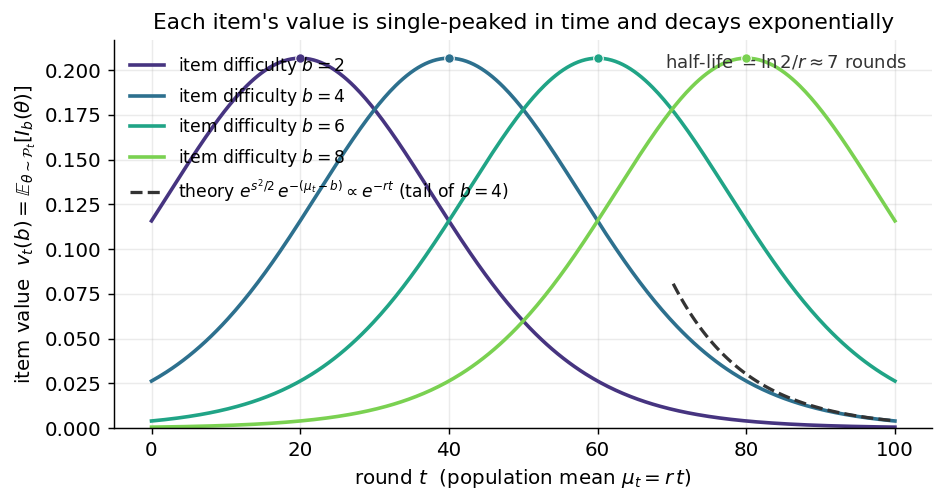
\includegraphics[width=0.82\textwidth]{fig1.png}
\caption{The decay law. Value $v_t(b)$ of questions at four difficulties as the
field's mean ability rises at rate $r$ (here $r=0.1$, $s=1$). Each curve rises as the
field approaches the question, peaks when the mean ability equals its difficulty
(dots), and decays exponentially after. The dashed line is the closed-form tail
$e^{s^2/2}e^{-(\mu_t-b)}\propto e^{-rt}$ of Proposition~\ref{prop:decay}. The
half-life is $\ln 2/r\approx 7$ rounds.}
\label{fig:decay}
\end{figure}

\subsection{The maintenance problem}
\label{sec:problem}

We want to rank the field well at every round. The error in a model's ability
estimate is, by standard theory, inversely proportional to the information collected
about it. So if a bank provides total information
\begin{equation}
\cI_t(\theta;\cB)=\sum_{i\in\cB}I_{b_i}(\theta)
\label{eq:totinfo}
\end{equation}
at ability $\theta$, ranking the whole field well means making this large everywhere
the field is. The natural single number is the field-averaged ability variance,
\begin{equation}
\Psi_t(\cB)=\int\frac{\rho_t(\theta)}{\cI_t(\theta;\cB)}\,d\theta,
\label{eq:psi}
\end{equation}
which we call the \emph{ranking error}: it is small when the bank covers the field
with information and large when it leaves gaps. The best one-round bank minimizes it
under a size budget.

\begin{problem}[Best bank at one round]
\label{prob:one}
Given the field $\cP_t$ and a budget of $N$ questions,
\begin{equation}
\min_{\cB\subset\cU,\ |\cB|\le N}\ \Psi_t(\cB).
\label{eq:prob1}
\end{equation}
Write $\cB^\star_t$ for a minimizer.
\end{problem}

\begin{remark}[Why not just maximize value?]
One might instead maximize total value $V_t$. But that is degenerate: since value is
a sum and each question's value peaks at one difficulty (near the field's mean), the
best bank would put every question at that one difficulty and leave strong and weak
models unresolved. The ranking error $\Psi_t$ avoids this, because a gap in coverage
(where $\cI_t\to 0$) sends the error to infinity. So $\Psi_t$ is the objective; value
and its decay law are the intuition for why the target moves.
\end{remark}

In practice three things make this harder than a one-round fit. The field
\emph{moves}~\eqref{eq:drift}, so the best bank changes; the bank can be changed only
\emph{slowly}, since new hard questions must be written; and the difficulties are
\emph{not known}, but estimated from the answers we collect. A maintenance method
must therefore choose, each round, both \emph{which answers to collect} (which
questions to retire, which to add, and which model answers which question) and
\emph{how to re-estimate difficulty} from those answers.

\begin{problem}[Online maintenance]
\label{prob:online}
Run a method that, each round $t$, selects the bank $\cB_t$ and collects answers,
then re-estimates difficulties, so as to keep the ranking error low at every round,
\begin{equation}
\text{minimize }\ \Psi_t(\cB_t)\ \text{ for all } t,\quad
\text{subject to }\ |\cB_t|\le N,\quad |\cB_t\setminus\cB_{t-1}|\le\kappa,
\label{eq:prob2}
\end{equation}
where $N$ bounds the bank size and $\kappa$ bounds how many \emph{new} questions can
be added per round (retiring questions is free; writing them is not). We measure
success by the gap to the one-round best, $\Psi_t(\cB_t)-\Psi_t(\cB^\star_t)$.
\end{problem}

\paragraph{Fixing the scale across time (a construction we will need).} The error
$\Psi_t$ compares models from round to round, so it needs one ability scale that
holds over time. The model~\eqref{eq:rasch} does not give one for free: only
differences $\theta_j-b_i$ appear, so shifting all abilities and difficulties by the
same amount, or stretching them together, leaves every answer probability unchanged.
Calibrating each round on its own therefore leaves the means $\mu_t$ incomparable
across rounds, and the drift rate $r$ undefined. We fix this with a set of
\emph{anchor questions} $\cA$ that are kept in the bank at all times and never
retired: administering them every round and holding their difficulties fixed pins
the scale, so that $\mu_t$ is comparable over time and $r$ is identified. This is the
one extra ingredient the algorithm relies on, and it is built into its first step.

\section{An Online Maintenance Algorithm}
\label{sec:algo}

We now give a method for Problem~\ref{prob:online} and prove it stays near-optimal.
We first describe the loop in words, then define its operations precisely, then
state the algorithm and the guarantee.

\paragraph{The loop, in words.} Each round, the method (i) gives every model a fixed
set of anchor questions plus a few questions matched to its level, and re-estimates
abilities on the anchor-fixed scale; (ii) updates the difficulty of every asked
question from the new answers; (iii) writes a few new hard questions and tries them
on the models nearest their level to calibrate them; and (iv) drops questions the
field has outgrown, keeping the bank at its size budget. The same answers do two
jobs---measuring models and calibrating questions.

\paragraph{Operations.} Algorithm~\ref{alg:main} calls five functions, each defined
here in full; $\tau,q,P_0>0$ are fixed constants.

\textit{Ability fit.} Given a model's difficulties and binary answers
$D=\{(b_i,u_i)\}_{i\in S}$,
\begin{equation}
\Fit(D):=\argmax_{\theta\in\R}\sum_{i\in S}\Bigl[u_i\log\sigm(\theta-b_i)
+(1-u_i)\log\bigl(1-\sigm(\theta-b_i)\bigr)\Bigr]-\frac{\theta^2}{2\tau^2},
\label{eq:fitop}
\end{equation}
the unique root of $\sum_{i\in S}\bigl(u_i-\sigm(\theta-b_i)\bigr)=\theta/\tau^2$;
solve by Newton's method.

\textit{Routing.} Given an ability $\theta$, a finite set $S$ with difficulties
$\{b_i\}_{i\in S}$, and a count $m\le|S|$, order the elements as
$|b_{i_1}-\theta|\le\cdots\le|b_{i_{|S|}}-\theta|$ (ties by index) and set
\begin{equation}
\Route(\theta,S,m):=\{i_1,\dots,i_m\},
\label{eq:route}
\end{equation}
the $m$ questions of nearest difficulty---the most informative available for that
model by~\eqref{eq:info}.

\textit{Difficulty filter.} Given a question's current estimate $(\hat b,P)$, a
model's ability $\hat\theta$, and that model's answer $u\in\{0,1\}$, set
$\hat p=\sigm(\hat\theta-\hat b)$ and define
$\Filter(\hat b,P;\hat\theta,u):=(\hat b',P')$ by
\begin{equation}
\tilde P=P+q,\qquad
\hat b'=\hat b+\frac{\tilde P}{1+\tilde P\,\hat p(1-\hat p)}\,(\hat p-u),\qquad
P'=\bigl(\tilde P^{-1}+\hat p(1-\hat p)\bigr)^{-1}.
\label{eq:filter}
\end{equation}
This is a Kalman update for a logistic answer: a model passing more often than
predicted ($u=1$, $\hat p<1$) lowers $\hat b$; the constant $q$ lets the estimate
follow slow drift.

\textit{Value.} Given the estimated field mean $\hat\mu$ and spread $\hat s$, the
value of a question of estimated difficulty $b$ (Definition~\ref{def:value} at the
estimated field) is
\begin{equation}
\hat v(b;\hat\mu,\hat s):=\int_{\R}I_b(\theta)\,\phi(\theta;\hat\mu,\hat s)\,d\theta,
\qquad
I_b(\theta)=\sigm(\theta-b)\bigl(1-\sigm(\theta-b)\bigr),
\label{eq:valueop}
\end{equation}
with $\phi(\cdot;\hat\mu,\hat s)$ the normal density---a one-dimensional integral,
evaluated by quadrature.

\textit{Acquisition.} A bank of $N$ questions over the live window of width
$\approx 4s$ has density $\delta\approx N/(4s)$ questions per unit of difficulty, so
adding $\kappa$ questions per round at the top raises the covered ceiling by the
\emph{acquisition rate}
\begin{equation}
a=\kappa/\delta\approx 4s\,\kappa/N\qquad\text{(ability units per round)}.
\label{eq:acqrate}
\end{equation}
Given a count $\kappa$ and a ceiling $c$, $\Acquire(\kappa,c)$ commissions $\kappa$
new questions targeting difficulties evenly spaced across the new band $[c,c+a]$:
question $\ell=1,\dots,\kappa$ enters the bank with initial state
\begin{equation}
\hat b^{(0)}_\ell=c+\frac{\ell-\frac12}{\kappa}\,a,\qquad P^{(0)}_\ell=P_0,
\label{eq:acqinit}
\end{equation}
a large uncertainty $P_0$, and is marked provisional; its true difficulty is unknown
and is learned by the filter~\eqref{eq:filter} from later answers.

\begin{algorithm}[t]
\caption{Online benchmark maintenance, round $t$}
\label{alg:main}
\textbf{Input:} bank $\cB_{t-1}$ with estimates $\{(\hat b_i,P_i)\}$, split into
trusted $\cB^{\mathrm{tr}}$ and provisional $\cB^{\mathrm{pr}}$; anchors
$\cA\subseteq\cB^{\mathrm{tr}}$; previous abilities $\{\hat\theta_{j,t-1}\}$; budgets
$N,\kappa,k,\nexp$; retirement threshold $\underline{v}$; promotion level $P^\star$.
\begin{enumerate}
\item \textbf{Select and ask.} For each model $j$, set
$Q^{\mathrm{tr}}_j=\Route(\hat\theta_{j,t-1},\cB^{\mathrm{tr}}\setminus\cA,\,k-\nexp)$
and $Q^{\mathrm{pr}}_j=\Route(\hat\theta_{j,t-1},\cB^{\mathrm{pr}},\nexp)$;
administer $Q_j=\cA\cup Q^{\mathrm{tr}}_j\cup Q^{\mathrm{pr}}_j$ and observe
$\{U_{ij}\}_{i\in Q_j}$.
\item \textbf{Estimate abilities and field.} For each $j$,
$\hat\theta_{j,t}=\Fit\bigl(\{(\hat b_i,U_{ij}):i\in\cA\cup Q^{\mathrm{tr}}_j\}\bigr)$;
then $\hat\mu_t=\frac1M\sum_j\hat\theta_{j,t}$ and
$\hat s^2_t=\frac{1}{M-1}\sum_j(\hat\theta_{j,t}-\hat\mu_t)^2$.
\item \textbf{Recalibrate.} For every asked pair $(i,j)$ with $i\notin\cA$:
$(\hat b_i,P_i)\leftarrow\Filter(\hat b_i,P_i;\hat\theta_{j,t},U_{ij})$.
\item \textbf{Promote and acquire.} Move each $i\in\cB^{\mathrm{pr}}$ with
$P_i\le P^\star$ into $\cB^{\mathrm{tr}}$; then add
$\cB^{\mathrm{new}}=\Acquire(\kappa,\hat\mu_t+2\hat s_t)$ to $\cB^{\mathrm{pr}}$.
\item \textbf{Retire and cap.} Drop every non-anchor $i$ with
$\hat v(\hat b_i;\hat\mu_t,\hat s_t)<\underline{v}$; if the bank still exceeds $N$,
drop the lowest-value non-anchors until $|\cB_t|\le N$.
\end{enumerate}
\textbf{Output:} bank $\cB_t$; abilities $\hat\theta_{\cdot,t}$; ranking
$\argsort(\hat\theta_{\cdot,t})$; and the winner $\argmax_j W_j$~\eqref{eq:winrate}
if a single one is wanted.
\end{algorithm}

\paragraph{The guarantee.} Recall the acquisition rate $a$ of~\eqref{eq:acqrate},
the speed at which step~5's writing pushes the covered ceiling upward, and the drift
rate $r$, the speed at which the field rises. The next result says the algorithm
keeps the benchmark as good as the one-round best at every round, exactly when it
can write hard questions fast enough.

\begin{theorem}[Algorithm~\ref{alg:main} stays near-optimal]
\label{thm:main}
Suppose the field's mean rises at rate $r$~\eqref{eq:drift}, the universe $\cU$
contains questions of every difficulty, and Algorithm~\ref{alg:main} runs with a
fixed anchor set $\cA$, size budget $N$, and acquisition budget $\kappa$, with
acquisition rate $a$ from~\eqref{eq:acqrate}. Then at every round $t$:
\begin{enumerate}
\item[(i)] (scale) the anchor set fixes the ability scale, so $\mu_t$ is comparable
over time and the drift $r$ is identified;
\item[(ii)] (gap) the gap to the one-round best splits as
$\Psi_t(\cB_t)-\Psi_t(\cB^\star_t)=\varepsilon^{\mathrm{cal}}_t+\varepsilon^{\mathrm{cov}}_t$,
where the \textup{calibration gap}
$\varepsilon^{\mathrm{cal}}_t=O(1/\sqrt{n_t})$ shrinks as questions gather $n_t$
answers, and the \textup{coverage gap} $\varepsilon^{\mathrm{cov}}_t$ stays bounded
for all $t$ if $a\ge r$ and grows like $(r-a)\,t$ if $a<r$.
\end{enumerate}
Hence Algorithm~\ref{alg:main} solves Problem~\ref{prob:online}---it keeps the
ranking error within a vanishing gap of the one-round best at all times---\textup{if
and only if} $a\ge r$, equivalently (by~\eqref{eq:acqrate}) the writing budget
satisfies $\kappa\ge rN/(4s)$.
\end{theorem}

\begin{proof}[Proof sketch]
(i) Holding the anchors' difficulties fixed removes the shift-and-stretch freedom
of~\eqref{eq:rasch}, so all rounds share one scale and $\mu_t$ can be compared; $r$
is then the slope of $\mu_t$ in $t$. \emph{(ii), coverage.} The window's top is at
$\mu_t+2s=\mu_0+2s+rt$, while the bank covers up to $\mathrm{cap}_0+at$. The part of
the field left uncovered has size $\max(0,(r-a)t+\mathrm{const})$. Where the bank
gives no coverage, $\cI_t\to 0$, so the integrand of $\Psi_t$~\eqref{eq:psi} blows up
there; the extra error grows with the uncovered part, which is bounded exactly when
$a\ge r$. \emph{(ii), calibration.} A new question's difficulty estimate concentrates
at the usual $1/\sqrt n$ rate in the answers it has gathered, and its shortfall in
information is of the same order, summing to a bounded per-round amount once
acquisition is steady.
\end{proof}

The message is blunt: a benchmark stays alive only if new hard questions are written
at least as fast as the field improves. If they are, the only remaining cost is the
small, fading error from not-yet-calibrated questions. If they are not, coverage
falls behind and the benchmark goes stale, no matter how well the existing questions
are re-fit or routed---which is the fate of a fixed benchmark. The practical content
of Theorem~\ref{thm:main} is a \emph{writing schedule}: add hard questions at rate
$a\ge r$. Writing questions, not compute, is the binding constraint.

\paragraph{One pool of answers, two jobs.} Algorithm~\ref{alg:main} measures models
and calibrates new questions from the same answers. Step~1 gives each model $k-\nexp$
trusted questions at its level, which measure it, and $\nexp$ provisional ones, which
calibrate the new questions; the abilities in step~2 use only the trusted answers, so
provisional miscalibration does not bias them. The single number $\nexp$ trades the
two jobs: at $\nexp=0$ models are measured sharply but new questions never get
calibrated; larger $\nexp$ calibrates new questions fast at a small cost to this
round's ranking. We see this trade in \S\,\ref{sec:exp}.

\section{Experiments}
\label{sec:exp}

We test the method on synthetic data: a field $\cN(\mu_t,s^2)$ with $\mu_t=rt$,
questions with known or filter-estimated difficulty, and abilities recovered
by~\eqref{eq:fit}. Ranking quality is the Spearman correlation between estimated and
true abilities of the current field, averaged over runs. Figure~\ref{fig:decay}
already showed the decay law; here we test the algorithm against
Problem~\ref{prob:online}.

\paragraph{A fixed benchmark decays; a maintained one does not.}
Figure~\ref{fig:fixed} runs three methods for 80 rounds at $r=0.1$. The fixed
benchmark never changes; the recalibrated one re-estimates its difficulties each
round but adds nothing; full maintenance retires easy questions and adds hard ones
(with bank size held fixed, so value reflects coverage, not count). The fixed
benchmark's value falls from 45 to near 0 as the field passes it, and its ranking
quality drops from 0.91 to 0.32. Recalibration does not help: its curve sits on the
fixed one, because a question everyone passes carries no information whether or not
we know its difficulty. Only full maintenance holds value ($\approx 45$) and ranking
($\approx 0.91$)---the difference between re-estimating questions and replacing them.

\begin{figure}[t]
\centering
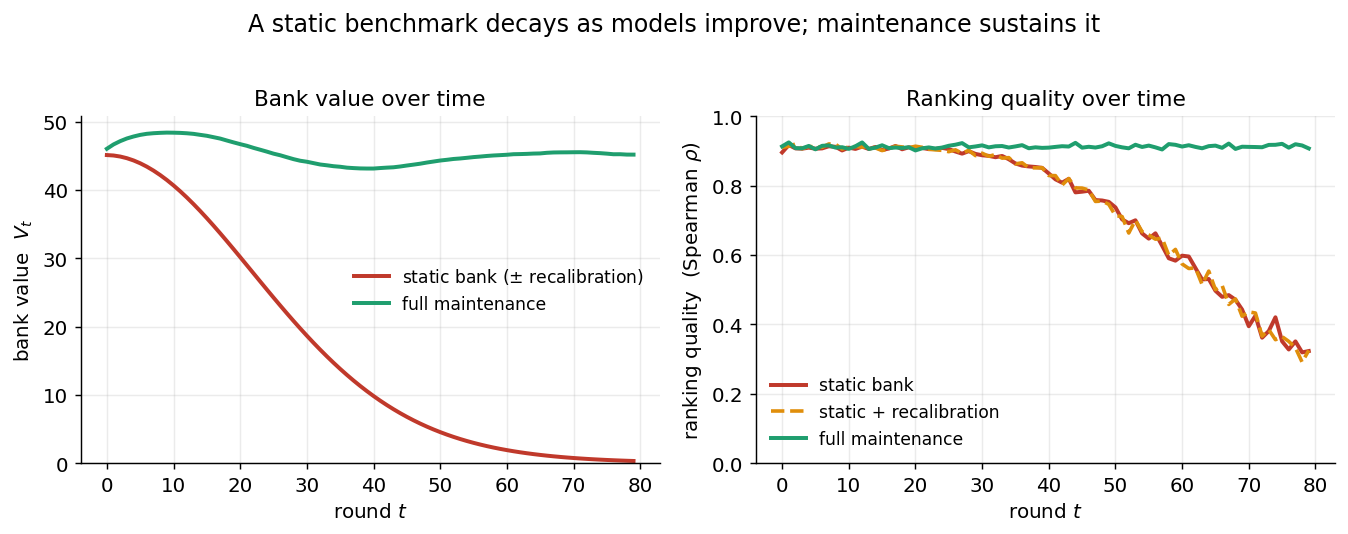
\includegraphics[width=\textwidth]{fig2.png}
\caption{Fixed versus maintained, at drift $r=0.1$. \textbf{Left:} bank value over
time---the fixed benchmark (with or without recalibration) decays to zero; full
maintenance holds it. \textbf{Right:} ranking quality---the fixed and recalibrated
benchmarks decay together; full maintenance holds.}
\label{fig:fixed}
\end{figure}

\paragraph{The benchmark survives exactly when writing keeps pace.}
Figure~\ref{fig:threshold} varies the acquisition rate $a$ against the drift rate $r$
and reports steady-state ranking quality. Below $a/r=1$ coverage falls behind and
quality drops---to 0.66 when no new questions are written. At and above $a/r=1$
quality plateaus near 0.90. The threshold at $a=r$ is exactly the condition of
Theorem~\ref{thm:main}.

\paragraph{One pool, two jobs, one knob.} Figure~\ref{fig:knob} checks efficiency.
The left panel shows measurement is cheap: routing each model to matched-difficulty
questions reaches a given ranking quality with fewer questions per model than random
sampling---at $k=14$, $\rho=0.955$ versus 0.936, the gap larger at small budgets. The
right panel turns the exploration knob $\nexp$: at $\nexp=0$ models are measured
sharply ($\rho=0.965$) but new questions never calibrate within the horizon
($\mathrm{lag}=40$ rounds); raising it calibrates new questions fast ($\nexp=9$:
$\mathrm{lag}\approx 2$) at a small cost to ranking ($\rho=0.924$). The two jobs
trade off along a clean curve.

The four results trace the argument: value decays with progress
(Figure~\ref{fig:decay}); a fixed benchmark therefore dies while a maintained one
survives (Figure~\ref{fig:fixed}); survival holds exactly when writing keeps pace
(Figure~\ref{fig:threshold}); and the method runs efficiently from one pool of
answers with a single trade-off (Figure~\ref{fig:knob}).

\begin{figure}[t]
\centering
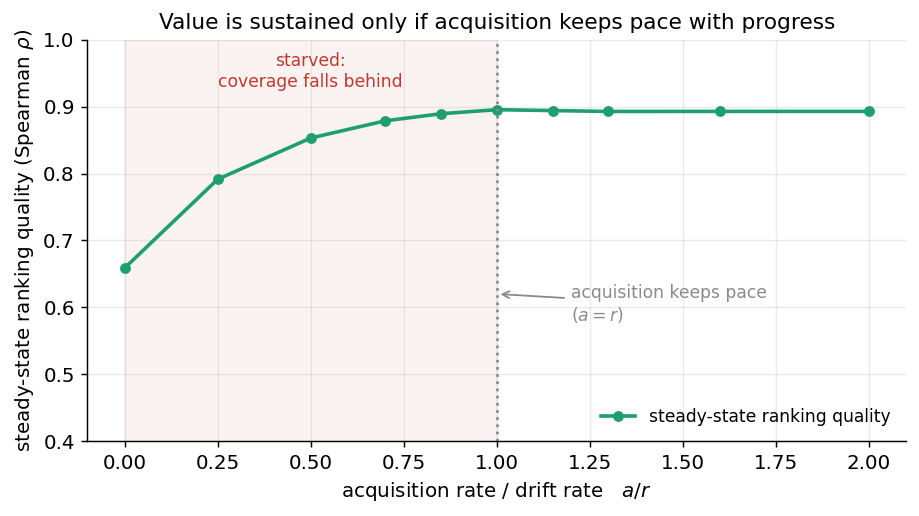
\includegraphics[width=0.72\textwidth]{fig3.png}
\caption{The survival threshold. Steady-state ranking quality against the ratio of
acquisition rate to drift rate $a/r$. Coverage falls behind for $a/r<1$ (shaded) and
is held for $a/r\ge 1$, matching Theorem~\ref{thm:main}.}
\label{fig:threshold}
\end{figure}

\section{Discussion}
\label{sec:disc}

\paragraph{Naming a single winner.} The maintained benchmark gives, each round, an
ability $\hat\theta_j$ for every model on a stable scale. When a single overall
winner is wanted, the natural summary is the \emph{average win-rate},
\begin{equation}
W_j=\frac{1}{M-1}\sum_{k\ne j}\mathbb{P}(\text{model } j \text{ beats model } k
\text{ on a random matched question}).
\label{eq:winrate}
\end{equation}
This is a definition, not a new method. Under the model~\eqref{eq:rasch}, the chance
that $j$ beats $k$ on a matched question rises with $\theta_j-\theta_k$, so $W_j$
rises with $\theta_j$ and the win-rate winner is the model with the highest ability.
Its worth is that, with scores made stable over time (this paper) and free of which
questions were asked (companion paper), an average win-rate is finally a fair basis
for naming a winner, not an artifact of the question mix or the moment of testing.

\begin{figure}[t]
\centering
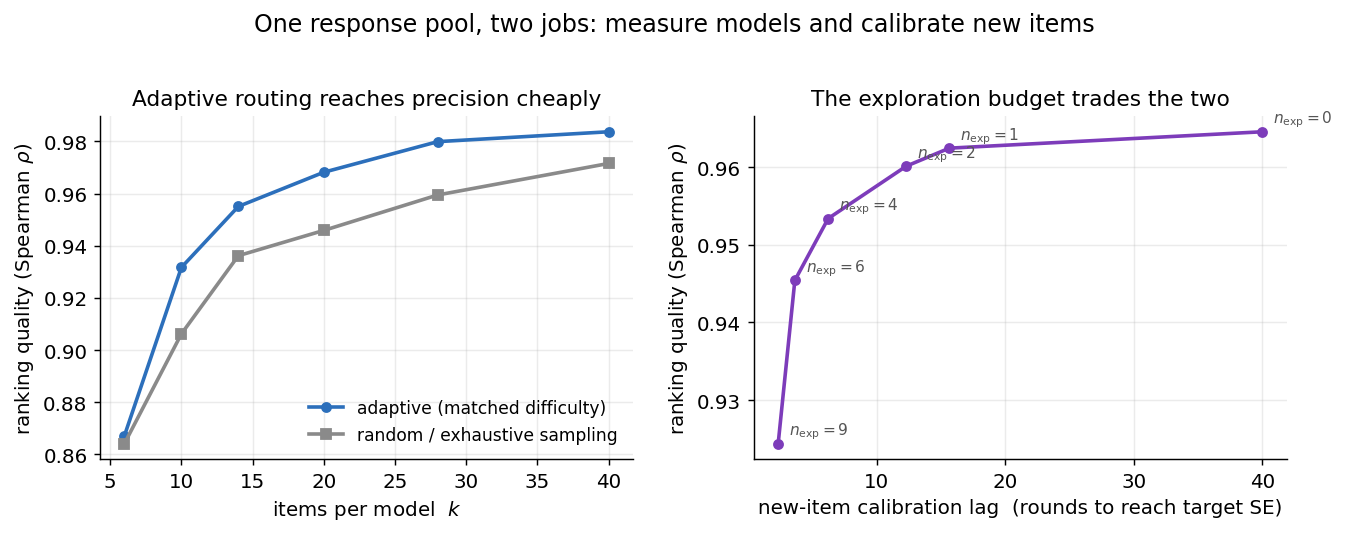
\includegraphics[width=\textwidth]{fig4.png}
\caption{Efficiency and the exploration knob. \textbf{Left:} matched-difficulty
routing reaches a target ranking quality with fewer questions per model than random
sampling. \textbf{Right:} the exploration budget $\nexp$ trades this round's ranking
quality (vertical) against how fast new questions calibrate (horizontal); points are
$\nexp=0,\dots,9$.}
\label{fig:knob}
\end{figure}

\paragraph{What a winner-rule rewards.} A single-winner rule is not a neutral readout
but a target the field will optimize toward. What it rewards can be read from where
its gradient is largest---improving there helps you win most---and from where the
field settles when everyone climbs that gradient. Table~\ref{tab:rules} compares the
average win-rate with two alternatives. The three differ in how they combine a
model's performance across tasks: the win-rate averages it (rewarding broad
competence), the medal count counts the tasks where the model is top (rewarding
peaks, and so specialists), and the worst-case keeps only its weakest task (rewarding
robustness, and so no blind spots)---mean, count, and minimum, pulling toward
breadth, spikes, and uniformity. All three are relative to the current field, so none
rewards absolute progress: a model that improves a lot can keep the same score if the
field improves with it. Rewarding absolute progress needs a fixed external
target---say, the fraction of held-out hard problems solved---which is exactly what a
time-stable scale and a steady supply of hard questions make possible.

\begin{table}[t]
\centering
\small
\begin{tabular}{@{}p{0.16\textwidth}p{0.19\textwidth}p{0.33\textwidth}p{0.19\textwidth}@{}}
\toprule
\textbf{Rule} & \textbf{Gradient largest on} & \textbf{Rewards (and its cost)} & \textbf{Induced ideal}\\
\midrule
Average win-rate $W_j$~\eqref{eq:winrate} &
close questions, where the field is split near your level; flat once you beat everyone &
broad ability \emph{relative to the field}, robust to single-test luck; weak pull past the pack, so it under-rewards extending the frontier &
a generalist that beats the current field everywhere\\[3pt]
Tasks won (medal count) &
tasks where you sit just below first &
peak skill on individual tasks, not breadth; needs the full profile, so it favors specialists &
a spiky model topping as many tasks as possible\\[3pt]
Worst-case (maximin) &
your single worst task only &
robustness and no blind spots; penalizes specialization and ignores peaks &
a model with no weaknesses---and no peaks\\
\bottomrule
\end{tabular}
\caption{Single-winner rules read as targets the field optimizes toward. A rule's
gradient marks where improvement most changes who wins; the induced ideal is the
model it rewards. The three differ in how they aggregate performance across tasks:
win-rate by averaging, medal count by counting the tasks led, worst-case by the
weakest task.}
\label{tab:rules}
\end{table}

\paragraph{Limits.} Three caveats bound the method. (i) \emph{The anchor set is
essential and self-undermining.} The anchors fix the scale, but they too become too
easy over time and cannot be frozen forever; in practice one refreshes them
gradually, introducing new anchors and tying them to the old ones before the old ones
are dropped, which slowly drifts the scale. (ii) \emph{Writing questions is the
binding constraint.} Theorem~\ref{thm:main} says the benchmark survives only if hard
questions arrive as fast as the field improves; for templated or model-generated
questions this is a writing schedule, but for human-written ones hard questions are
scarce, and no amount of re-fitting substitutes for them. (iii) \emph{The field and
the questions are estimated together.} The method estimates a moving field and
moving questions against each other; the fixed anchors are what break the
circularity, which is why their integrity matters most.

\paragraph{Summary.} A question's value is single-peaked in time and decays
exponentially once the field passes it, at the speed of progress. Keeping a benchmark
useful is therefore an ongoing task, not a one-time build: keep anchors to fix the
scale, re-estimate question difficulty from answers, drop questions that have become
too easy, and---above all---write new hard questions fast enough to keep up with the
field. Do that, and the benchmark keeps ranking a rising field; with scores stable
over time, an average win-rate finally names a winner that means what it says.

\end{document}
